\section{Evaluation}
\label{sec:evaluation}
\begin{figure*}[t]
        \centering
        \begin{subfigure}[b]{0.3\textwidth}
                \centering
                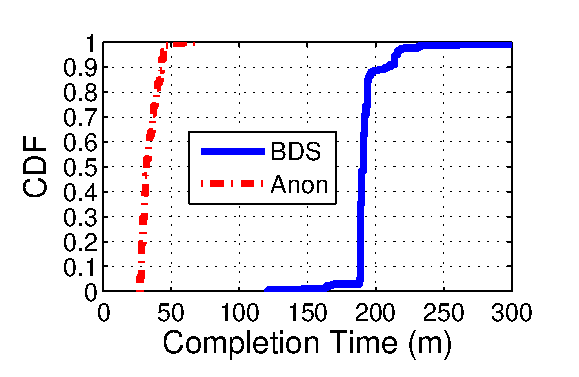
\includegraphics[width=\textwidth]{images/BDSvsAnon_overall.eps}
                \caption{Distribution of completion time.}
                \label{fig:BDSvsAnon:overall}
        \end{subfigure}
        \begin{subfigure}[b]{0.3\textwidth}%@X:\6 PieBridge\simulation\beijing\3 Applications\plot
                \centering
                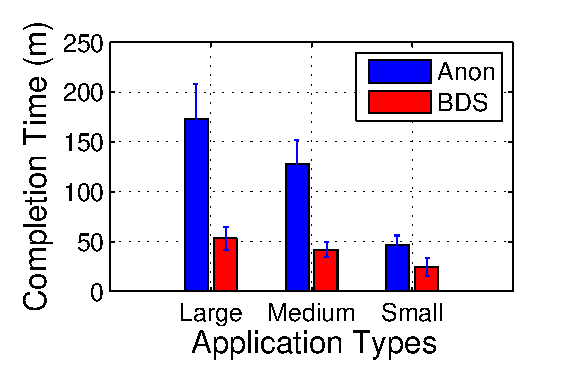
\includegraphics[width=\textwidth]{images/BDS_VS_ANON_v3.eps}
                \caption{Comparison by application types.}
                \label{fig:BDSvsAnon:FCT}
        \end{subfigure}
        \begin{subfigure}[b]{0.3\textwidth}
                \centering
                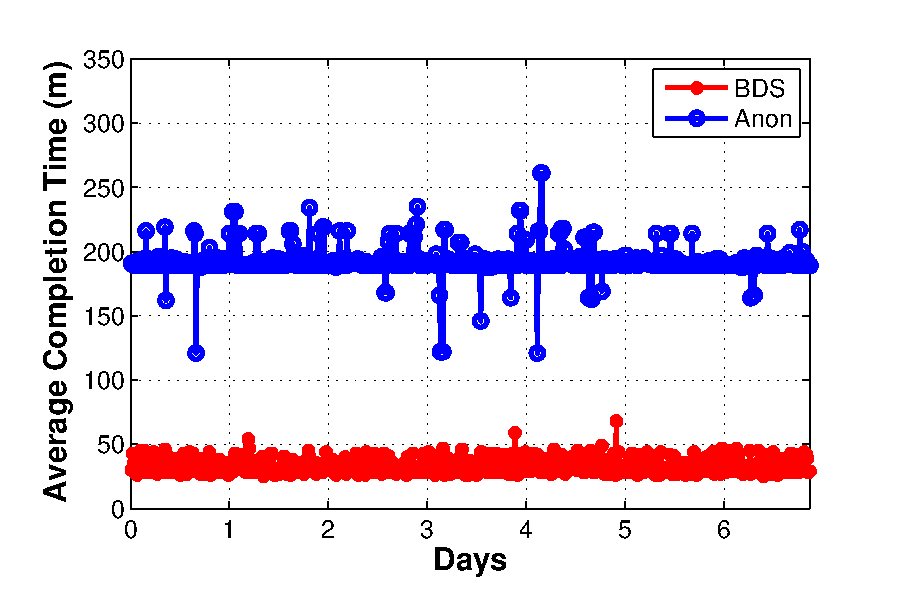
\includegraphics[width=\textwidth]{images/BDSvsAnon_time.eps}
                \caption{Comparison by completion time.}
                \label{fig:BDSvsAnon:time}
        \end{subfigure}
        \tightcaption{[\name vs. \company] Results from pilot deployments.}
        \label{fig:BDSvsAnon}
\vspace{-0.4cm}
\end{figure*}

To evaluate \name, we integrated our end-to-end prototype in \company, and ran a pilot deployment under the above implementation.
Using a combination of pilot deployment, trace-driven simulation, and microbenchmarking, we show that:
\begin{packedenumerate}
\item \name completes inter-DC multicast 3-5$\times$ faster than \company's existing solution and other baselines used in industry (\Section\ref{subsec:evaluation:centralized}).
\item \name significantly reduces the incidents of interferences between bulk-data multicast traffic and latency-sensitive traffic (\Section\ref{subsec:evaluation:separation}).
\item \name can scale to the traffic demand of a large online service provider, tolerate various failure scenarios, and is close to the theoretically optimal performance (\Section\ref{subsec:evaluation:benchmarks}).
\end{packedenumerate}

%\begin{figure*}[t] %@X:\6 PieBridge\simulation\DrawFig
%        \centering
%        \begin{subfigure}[b]{0.3\textwidth}
%                \centering
%                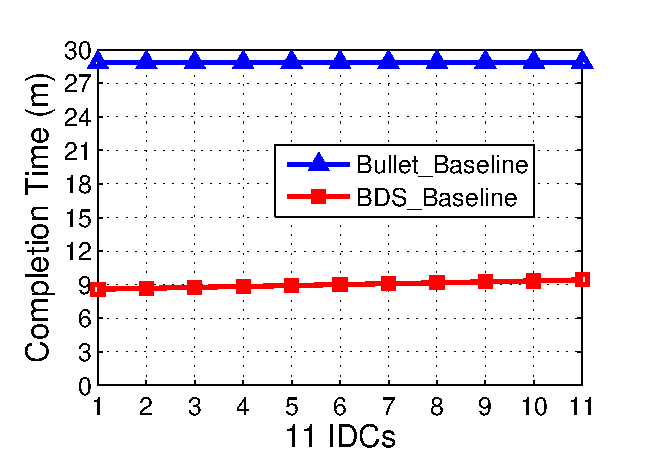
\includegraphics[width=50mm]{images/Test1.eps}
%                \caption{Baseline experiment.}
%                \label{fig:cdn:baseline}
%        \end{subfigure}
%        \begin{subfigure}[b]{0.3\textwidth}
%                \centering
%                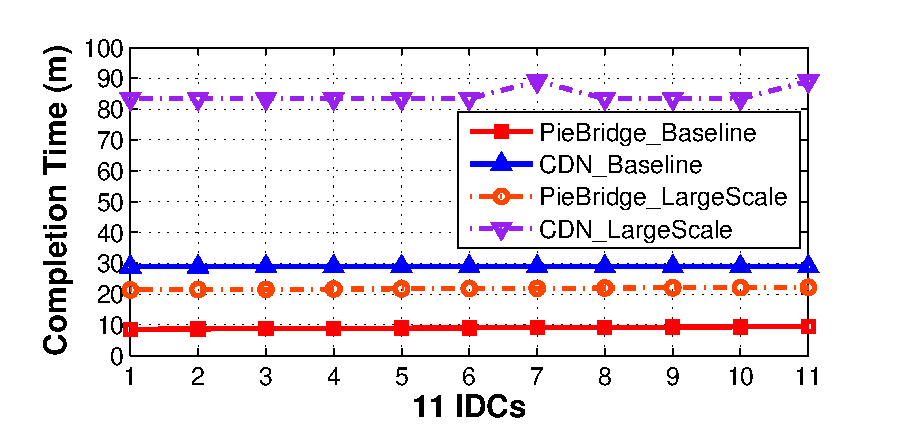
\includegraphics[width=50mm]{images/Test2.eps}
%                \caption{Large scale experiments.}
%                \label{fig:cdn:scale}
%        \end{subfigure}
%        \begin{subfigure}[b]{0.3\textwidth}
%                \centering
%                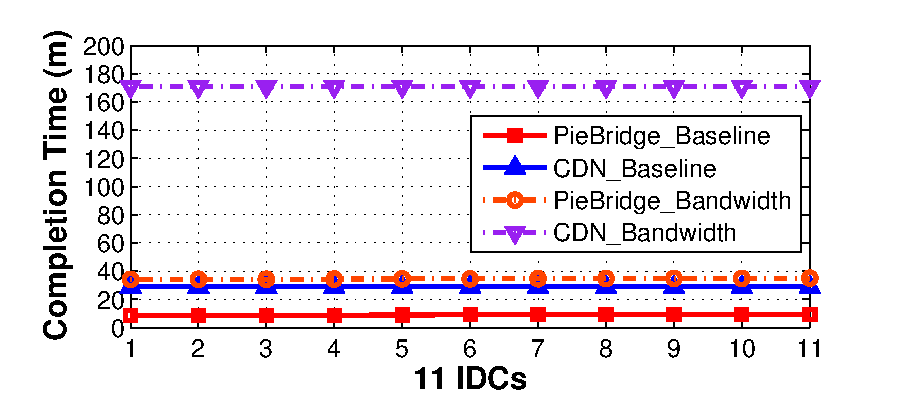
\includegraphics[width=50mm]{images/Test3.eps}
%                \caption{Small bandwidth experiments.}
%                \label{fig:cdn:bw}
%        \end{subfigure}
%        \caption{[\name versus Bullet] Comparisons under different network scenarios.}
%        \label{fig:versusCDN}
%\vspace{-0.4cm}
%\end{figure*}


\subsection{Performance improvement over existing solutions}
\label{subsec:evaluation:centralized}

We compare \name against three existing solutions:
\company's existing solution (a decentralized strategy which has been evolving for 5 years with end-to-end evaluations),
Bullet~\cite{kostic2003bullet} (a centralized strategy), and
Akamai's overlay network~\cite{Andreev2013Designing} for live video streaming
multicast.


\tightsubsubsection{Methodology}
We start with the methodology.

\mypara{Pilot deployment} We choose several services with different data sizes and run randomized A/B testing in which
%In general, such bulk data is transferred using \company's existing solution (that has already run for more than 5 years), while
we randomly choose several days to use \name instead of the current solution. To make sure that the two solutions work in the similar environment, we conduct all the experiments at 02:00 every day in the morning.

\mypara{Trace-driven simulation} Complementary to the pilot deployment on real traffic, we also use trace-driven simulation to evaluate \name on a larger scale.
%than the pilot deployment cannot implement other solutions on \company's real network. Instead,
We simulate the other two overlay multicast techniques by setting topology, DC scale and configuring servers with the same scale as \name's DCs, and replay inter-DC multicast data requests in the same chronological
order as in the pilot deployment (including the number of requests and the number of nodes).


%To evaluate the benefits of centralized control, we conduct two series of experiments: the comparisons with \company's existing solution based on the pilot deployments, and the comparisons with other overlay multicast techniques using trace-driven simulations.

\tightsubsubsection{\name vs. \company's existing solution}

We first choose one service with 70~TB aggregated daily bulk data, which is distributedly stored in the source DC. Each of the other DCs downloads a copy of the data and stores it in the same distributed way.

%First of all, we present the completion time of destination servers under \name and \company in Figure

To intuitively present the overall improvements by \name, we draw the cumulative distribution function (CDF) of the completion time in Figure \ref{fig:BDSvsAnon:overall}, from which we can see that the completion time under \company's existing solution is about 200 minutes while that under \name is less than 40 minutes, which is 5 times shorter.

For detailed illustration, we further pick three applications whose data volumes are large, medium and small, and compare \name's and \company's mean (stddev) completion time for each application in Figure \ref{fig:BDSvsAnon:FCT}.
%draw three pairs of bar charts in Figure \ref{fig:BDSvsAnon:FCT}, each representing \name's and \company's mean (stddev) completion time for one application.
These bars show that the benefit of \name increases along with the bulk data size. For small data volume, \name outperforms \company by 1.6 times, and more than 3 times than \company for large-data transfers.

We also repeat the experiments for 7 days to offer more statistical significance and draw the average completion time of both \name and \company in Figure \ref{fig:BDSvsAnon:time}. \name consistently outperforms \company by 4 times, and has less performance variations.
%is quite stable during these 7 days while \company illustrates some volatilities.
In general, \name achieves about 4.5 times shorter completion time than \company.
%\item \name vs. \company's existing solution (pilot deployment)
%\begin{itemize}
%\item Overall improvement: A CDF with two lines to show the aggregated flow completion time
%\item By applications: Pick three applications whose data volumes are large, medium, and small respectively. Draw a bar chart of three pairs of bars, each representing \name's and \company's mean (stddev) flow completion time for an application.
%\item By time: Timeseris of two lines, each representing \name's and \company's mean (stddev) of flow completion time.
%\end{itemize}

\tightsubsubsection{\name vs. other overlay multicast techniques}

%As we cannot implement other experimental systems in our real online network just as comparisons, we conduct a series of simulations using trace-driven simulations in this section, and compare \name's performance versus Bullet \cite{kostic2003bullet} and a CDN-based solution \cite{Andreev2013Designing} adopted by Akamai.

For \company's infrastructure, there are 1k to 20k servers in each DC, but there is no need for \name to be deployed in all the servers because only some of these servers are used for bunk data transfer. In the trace-driven simulations, we use a topology with 11 DCs (one of which acts as the source DC) and set all the parameters to be the same as for the real network, including data file size, data source and destination, paths, link capacities and server upload/download rates. We use two baselines: Bullet \cite{kostic2003bullet} is a data dissemination system using an overlay mesh, and Akamai's video streaming system \cite{Andreev2013Designing} in overlay multicast networks.

%We conduct three series of experiments and show the results in Figure \ref{fig:versusCDN}: baseline \ref{fig:cdn:baseline}, large scale \ref{fig:cdn:scale} and small bandwidth experiments \ref{fig:cdn:bw}. We find \name achieves 3$\times$ shorter completion time than Bullet in the baseline experiments, and more than 4$\times$ improvement in the large scale experiments and small bandwidth experiments.
We conduct three series of experiments and show the results in Table \ref{table:versusAkamai}: baseline, large-scale and small bandwidth experiments. In the baseline experiments, the size of the bulk data is 10TB, the number of servers per DC is 100, and the upload and download rate limits are set to 20MBs. In the large-scale experiment, the bulk data is 100TB, server number per DC is 1000. In the small bandwidth experiment, server upload and download rate limit are reduced to 5MBs. We find that \name achieves 3 times shorter completion time than Bullet and Akamai in the baseline experiments, and more than 4 times shorter completion time in the large-scale and small bandwidth experiments.

Considering the results in large-scale experiments, we found that the completion time of Bullet (and Akamai) increase to more than 3 times compared that in the baseline experiments - from $28m$ (and $25m$)to about $82m$ (and $87m$), while \name only increases to about 2 times - from $9.41m$ to $20.33m$. This proves \name's good scalability. Similarly, in the small bandwidth experiments (which is very common when delay-sensitive traffic bursts), the completion time of Bullet and Akamai increases to $171m$ and $138m$, respectively, while that of \name is just $38.25m$. This result illustrates the high efficiency of \name under strict bandwidth limitations.
%In the large scale experiments, the completion time of Bullet increases to about 3 times than that in the baseline experiment, and that of Akamai multicast solution is about 3.5 times. But \name., \name increase to while that of respectively.

\begin{table}[t]
\begin{center}
\resizebox{3in}{!}{
%\begin{tabular}{p{2cm}<{\centering}|p{2cm}<{\centering}}
\begin{tabular}{| c | c| c| c|}
\hline
 \rowcolor[gray]{0.9}
\textbf{Solution} & \textbf{Baseline} & \textbf{Large Scale} & \textbf{Rate Limit} \\
\hline \hline
Bullet & $28m$ & $82m$ & $171m$\\
\hline
Akamai & $25m$ & $87m$ & $138m$\\
\hline
\name & $9.41m$ & $20.33m$ & $38.25m$\\
\hline
\end{tabular}
}
\end{center}
\tightcaption{[\name vs. Bullet \cite{kostic2003bullet}, Akamai \cite{Andreev2013Designing}] Completion time of the three solutions in  trace-driven simulation.}
%\caption{Average completion time of Bullet \cite{kostic2003bullet}, Akamai \cite{Andreev2013Designing} and \name.}
\label{table:versusAkamai}
\vspace{-0.4cm}
\end{table}

%\begin{itemize}
%\item \name vs. other overlay multicast techniques
%\begin{itemize}
%\item Begin with the methodology of trace-driven simulation.
%\item Briefly explain these techniques: Akamai (3-layer), Bullet (full mesh)
%\item Show a CDF that has three lines, representing \name, Akamai, and Bullet.
%\end{itemize}
%\end{itemize}

\subsection{Benefits of coordinated bandwidth allocation}
\label{subsec:evaluation:separation}
\begin{figure}[t]
  \centering
  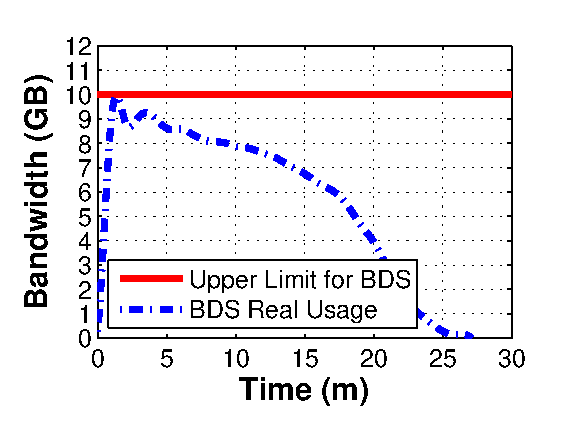
\includegraphics[width=45mm]{images/Quota_v2.eps}%DrawLink.m
  \tightcaption{The effectiveness of bandwidth separation.}
  \label{fig:quota}
\vspace{-0.4cm}
\end{figure}

To test the effectiveness of bandwidth separation and check whether the bulk data transfers affect latency-sensitive traffic, we set the upper bound of available bandwidth for bulk data transfer to 10~GBs, and monitor the real usage of one inter-DC link. The results are shown in Figure \ref{fig:quota}, from which we can see the real bandwidth usage stays below 10~GBs throughout the whole transmission process.
When being used online, the upper bound of bandwidth for bulk data transfers is set to be the difference between link capacity and the peak bandwidth of latency-sensitive workloads. Therefore, the effectiveness of \name bandwidth separation can guarantee that bulk transfers do not interfere with latency-sensitive workloads.% bound the bunk data transfer, the latency-sensitive workloads would generally not be interfered.
%and thus \name can effectively reduce the incidents of delay on latency-sensitive traffic caused by bulk data transfers.

\begin{table}[t]
\begin{center}
\resizebox{3in}{!}{%
%\begin{tabular}{p{2cm}<{\centering}|p{2cm}<{\centering}}
\begin{tabular}{| c | c | c | c | c |}
\hline
 \rowcolor[gray]{0.9}
\textbf{System} & \textbf{Source DC egress link} & \textbf{$l_1$} & \textbf{$l_2$} & \textbf{$l_3$}\\
\hline \hline
\company & 69.82\% & 53.09\% & 57.98\% & 63.01\% \\
\hline
\name & 70.55\% & 62.46\% & 63.23\% & 64.24\% \\
\hline
\end{tabular}
}
\end{center}
\tightcaption{Average link utilizations of the source DC egress link and 3 inter-DC links ($l_1$, $l_2$, $l_3$) under \company and \name.}
\label{table:usage}
\vspace{-0.4cm}
\end{table}

\begin{figure*}[t]
        \centering
        \begin{subfigure}[b]{0.3\textwidth}
                \centering
                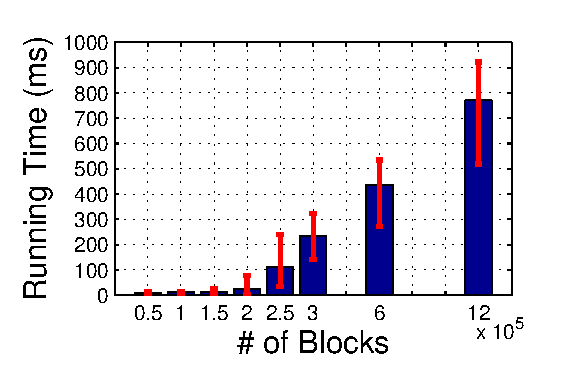
\includegraphics[width=50mm]{images/CPUvsBlk_v3.eps}% cpu.m replaced by running_time.m
                \caption{The controller running time.}
                \label{fig:scale:cpu}
        \end{subfigure}
        \begin{subfigure}[b]{0.3\textwidth}
                \centering
                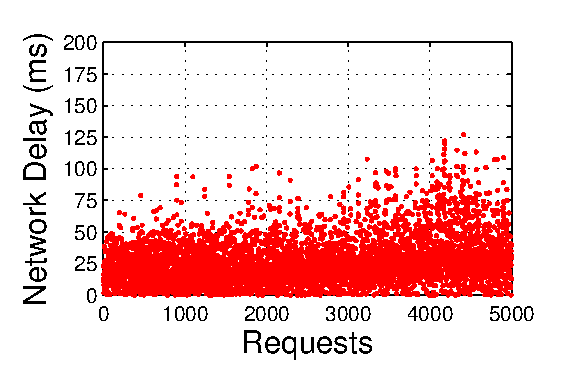
\includegraphics[width=50mm]{images/NetworkDelay.eps}%CDFofNetworkDelay -> Communication.m
                \caption{The inter-DC network delay.}
                \label{fig:scale:network}
        \end{subfigure}
        \begin{subfigure}[b]{0.3\textwidth}
                \centering
                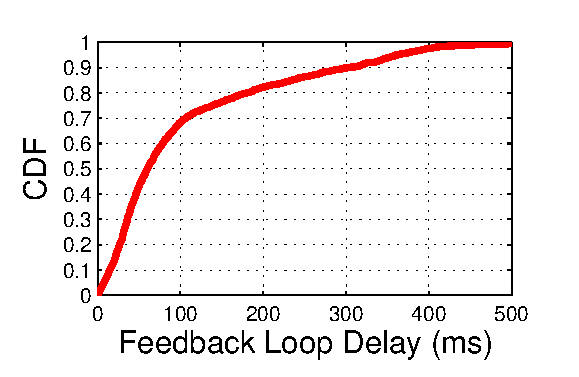
\includegraphics[width=50mm]{images/CDFofFeedbackLoopDelay.eps}
                \caption{Feedback loop delay.}
                \label{fig:scale:feedback}
        \end{subfigure}
        \tightcaption{[System scalability] Measurements on (a) controller running time, (b) network delay, (c) Feedback loop delay.}
        \label{fig:scale}
\vspace{-0.4cm}
\end{figure*}

\begin{figure*}[t]
        \centering
        \begin{subfigure}[b]{0.3\textwidth}
                \centering
                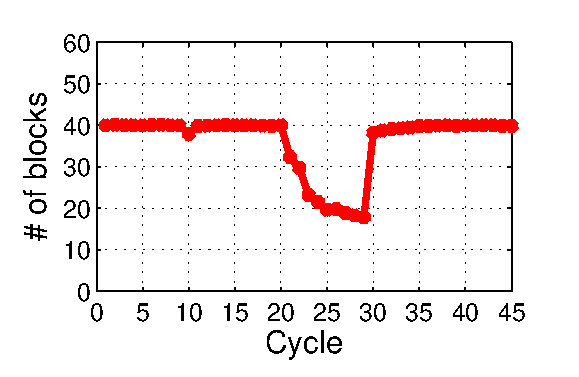
\includegraphics[width=50mm]{images/failure_v2.eps}%fail.m
                \caption{Average number of downloaded blocks per cycle under failures.}
                \label{fig:analysis:failure}
        \end{subfigure}
        \begin{subfigure}[b]{0.3\textwidth}
                \centering
                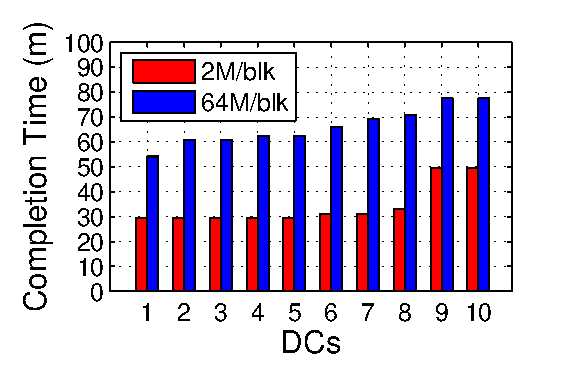
\includegraphics[width=50mm]{images/blkSize_v2.eps} %plotTCT_IDC.m
                \caption{Completion time under different block sizes.}
                \label{fig:analysis:blksize}
        \end{subfigure}
        \begin{subfigure}[b]{0.3\textwidth}
                \centering
                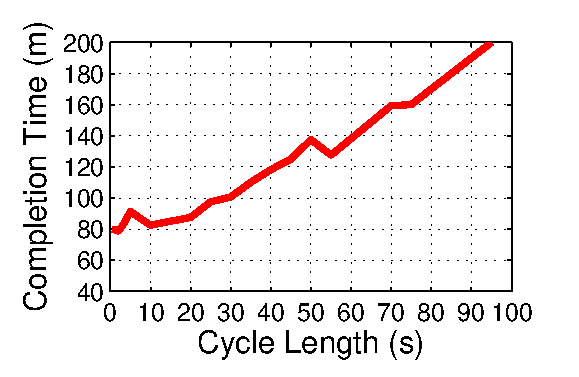
\includegraphics[width=50mm]{images/cycleDiff.eps}%cycleDiff.m
                \caption{Completion time under different cycle lengths.}
                \label{fig:analysis:cycleDiff}
        \end{subfigure}
%        \begin{subfigure}[b]{0.3\textwidth}
%                \centering
%                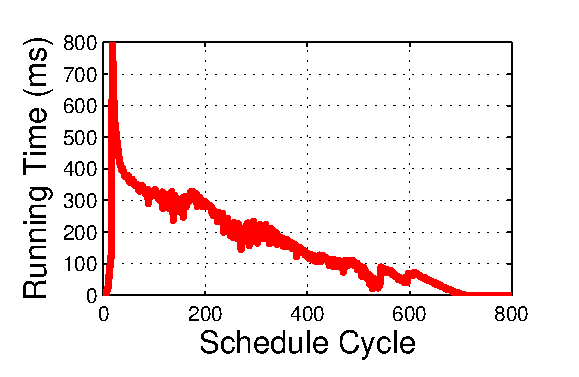
\includegraphics[width=50mm]{images/cycle.eps} %calculation_origin
%                \caption{Reduction on algorithm running time due to approximation.}
%                \label{fig:analysis:time}
%        \end{subfigure}
%        \begin{subfigure}[b]{0.3\textwidth}
%                \centering
%                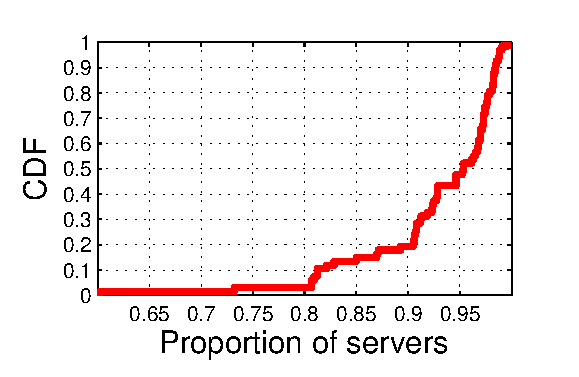
\includegraphics[width=50mm]{images/overlay.eps}
%                \caption{The proportion of blocks downloaded from the original source.}
%                \label{fig:analysis:overlay}
%        \end{subfigure}
        \tightcaption{\name's (a) fault tolerance, (b) sensitivity to different block sizes, and (c) different cycle lengths.}
        \label{fig:analysis}
\vspace{-0.4cm}
\end{figure*}


As \name implements strict bandwidth separation between latency-sensitive traffic and bulk data transfers while still showing shorter completion time, does it occupy too much bandwidth on inter-DC links? To answer this question, we record the average utilizations of the egress link of the source DC and 3 randomly selected inter-DC links, denoted as $l_1,l_2$ and $l_3$. The result in Table \ref{table:usage} shows that link utilizations do not change much with \name. This is because \name spreads data transfers over bottleneck-disjoint paths, so it avoids transferring the same data on the same link.

%\begin{itemize}
%\item Draw a graph (what graph can you get on this?) to show with bandwidth separation, \name can reduce the incidents of delay on latency-sensitive traffic caused by bulk data transfers.%DrawLink.m
%\item Draw a graph (what graph can you get on this?) to show the link utilization does not change much with \name or with \company.%DrawUsage.m
%\end{itemize}

\subsection{Micro-benchmarks}
\label{subsec:evaluation:benchmarks}

This section examines \name in very details through micro-benchmarks.
%focuses on some benchmarks of \name.
(1) Scalability of the centralized control.
%As \name adopts centralized control, the running time and scalability of the controller are key indicators of algorithm efficiency.
(2) Fault tolerance.
%Algorithm adaptability. \name runs together with latency-sensitive traffic, so high fault tolerance and strong robustness are essential requirements especially in rapidly changing networks. (3). In-depth analysis. The near-optimality of \name and the effects of exploring overlay networks also need to be clarified.
(3) Setting of \name parameters.

\tightsubsubsection{Scalability}\label{subsec:evaluation:benchmarks:scalability}

\mypara{Controller running time} As the controller needs to assign specific transmissions for all blocks, the algorithm running time is naturally related to the number of blocks. We show the relationship of block number and algorithm running time in Figure \ref{fig:scale:cpu}, from which we can see that the controller running time is still lower than $300ms$ even when there are $3\times 10^5$ blocks \myfootnote{$3\times 10^5$ is the instantaneous peak value of block number for a particular large scale CDN service, and $300ms$ is quite reasonable for practical usage.}. This is the instantaneous peak value of block number when the bulk data size is 10~TB, and the block merging scheme described in \Section\ref{subsec:system:centralized} will further reduce the block number and reduce the algorithm running time.

\mypara{Network delay} \name works in inter-DC networks, so the network delay among DCs is a key factor in the algorithm updating process. We record the network delay of 5000 requests and present the CDF in Figure \ref{fig:scale:network}. We can see that 90\% of the network delays are below $50ms$ and the average value is about $25ms$, which is less than 1\% of the decision updating cycle (3 seconds).

\mypara{Feedback loop delay} For centralized algorithms, a small feedback loop delay is essential to algorithm scalability. In \name, this feedback loop consists of several procedures: status updating from agents to the controller, running of the centralized algorithm, and decision updating from the controller back to agents. We measure the delay of the whole process, show the CDF in Figure \ref{fig:scale:feedback}, and find that in most cases (over 80\%), the feedback loop delay is lower than $200ms$. So we can claim that \name demonstrates a short enough update delay and is able to scale to even larger systems.

\begin{figure*}[t]
        \centering
        \begin{subfigure}[b]{0.3\textwidth}
                \centering
                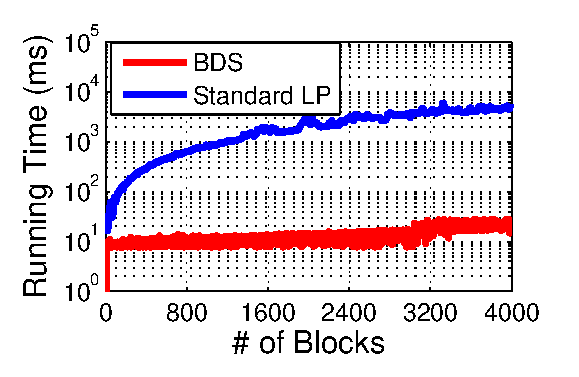
\includegraphics[width=50mm]{images/BDSvsLP_v2.eps} % BDSvsLP.m
                \caption{The reduction on algorithm running time of \name over standard LP.}
                \label{fig:further:BDSvsLP}
        \end{subfigure}
        \begin{subfigure}[b]{0.3\textwidth}
                \centering
                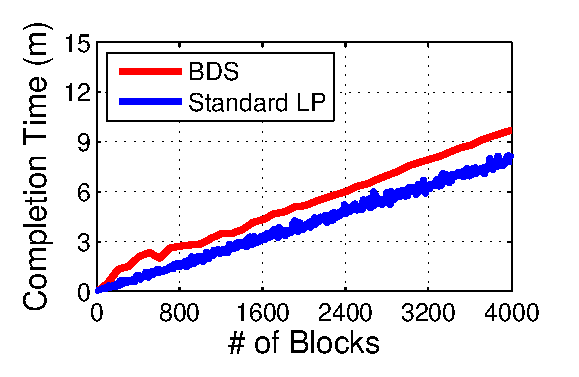
\includegraphics[width=50mm]{images/BDSvsLP_CT.eps}%BDSvsLP_CT -> Communication.m
                \caption{The near-optimality of \name to standard LP in small scale.}
                \label{fig:further:BDSvsLP_CT}
        \end{subfigure}
        \begin{subfigure}[b]{0.3\textwidth}
                \centering
                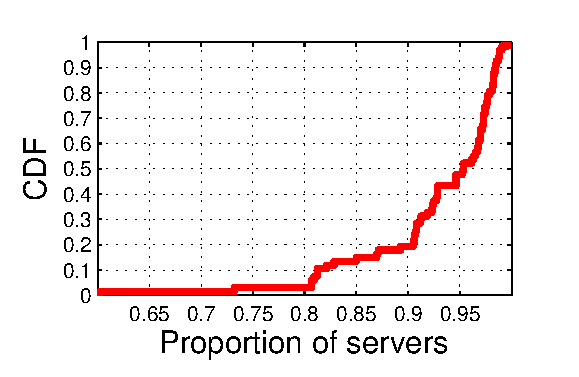
\includegraphics[width=50mm]{images/overlay.eps}
                \caption{The proportion of blocks downloaded from the original source.}
                \label{fig:further:overlay}
        \end{subfigure}
        \tightcaption{[In-depth analysis] on (a) reduction on algorithm running time, (b) near-optimality, and (c) effects of overlay transmission.}
        \label{fig:further}
\vspace{-0.4cm}
\end{figure*}

%\tightsubsubsection{Algorithm adaptability.}\label{subsubsec:evaluation:adaptability}
\tightsubsubsection{Fault tolerance}

%\mypara{Fault tolerance}
Here we examine the impact of the following failure scenario on the number of downloaded blocks per cycle. During cycles 0 to 9, \name works as usual, and one agent fails in the 10th cycle. The controller fails in the 20th cycle and recovers in the 30th cycle. Figure \ref{fig:analysis:failure} shows the average number of downloaded blocks per cycle. We find that the slight impact of agent failure only lasts for one cycle, and the system recovers in the 11th cycle. When the controller is unavailable, \name falls back to a default decentralized overlay protocol, resulting in graceful performance degradation. With the recovery of the controller, the performance recovers in the 30th cycle.

\tightsubsubsection{Choosing the values of key parameters}\label{subsec:evaluation:benchmarks:parameters}

\mypara{Block size} In \name, the bulk data file is split into blocks and can be transferred on bottleneck-disjoint paths. But this introduces a tradeoff between scheduling efficiency and calculation overhead. We therefore conduct two series of experiments using different block sizes (2MB and 64MB). Figure \ref{fig:analysis:blksize} shows that the completion time in the 2MB/block scenario is 1.5 to 2 times shorter than that in the 64MB/block scenario. This is because a smaller block sizes result in closer-to-optimal performance (see Appendix for the proof). However, this optimization introduces longer controller running time, as shown in Figure \ref{fig:scale:cpu}. We pick block size by balancing two considerations: (1) requirements on the completion time, and (2) controller's operation overhead.

\mypara{Update cycle lengths} Since any change in network environment may potentially alter the optimal overlay routing decisions, \name reacts to the changing network conditions by adjusting the routing scheme periodically. To testify the adjustment frequency, we set different cycle lengths from $0.5s$ to $95s$ to the same bulk data transfer, and Figure \ref{fig:analysis:cycleDiff} shows the completion time. Smaller cycle lengths result in shorter completion time, but the benefit diminishes when the cycle length is less than $3s$. This is because too frequent updates introduce more overhead on: (1) the information collection from agents to the controller, (2) the execution of the centralized algorithm, and (3) the re-establishment of new TCP connection. Thus, considering adjustment granularity and the corresponding overhead, we finally choose $3s$ as the default cycle length.


\tightsubsubsection{In-depth analysis.}\label{subsubsec:evaluation:depth}

\mypara{Optimization over algorithm running time} \name decouples scheduling and routing, which can significantly reduce the computational complexity. To clearly show the optimization, we measure the algorithm running time under \name and the standard linear programming (LP) solution. For the standard LP experiments, we use the \textit{linprog} library on MATLAB \cite{mathworks}, set the upper bound of the iteration number ($10^6$) if the algorithm does not converge, and record the CPU time as a function of the block number. Figure \ref{fig:further:BDSvsLP} shows that the running time of \name keeps below $25ms$ while that of standard LP grows quickly to $4s$ with only 4000 blocks. %This result illustrates \name's optimization over algorithm running time.
\name is much faster than off-the-shelf LP solver.

\mypara{Near-optimality of \name} To measure the near-optimality, we evaluate the data transfer completion time under the standard LP and \name: 2 DCs, 4 servers, 20MBs for server upload/download rate.
%1 to 4000 blocks (we cannot conduct large-scale experiments due to the explosive growth of the LP calculation time).
We vary the number of blocks from 1 to 4000, over which the LP solver can't finish in reasonable time. Figure \ref{fig:further:BDSvsLP_CT} shows that the difference of completion time between \name and the optimal standard LP is about 15\%.


\mypara{Benefit of disjoint overlay paths} \Section\ref{subsec:motivation:case-for} reveals the benefits of disjoint paths on application-level overlay networks. To explore the potential benefit, we record the ratio of the number of blocks downloaded from the original source to the total number of blocks, and the CDF is shown in Figure \ref{fig:further:overlay}. For about 90\% servers, the proportion is less than 20\%, which means that more than 80\% blocks are downloaded from other DCs on the disjoint paths, demonstrating great potential of multicast overlay network.

%\mypara{Breakdown of feedback loop delay} \name also applies the approximation of separating data scheduling from overlay routing, which can also reduce algorithm running time. We show the measurements on algorithm running time in Figure \ref{fig:analysis:time}. At the very beginning, the running time is nearly $800ms$, but drops to $300ms$ and even less quickly. This is because the separated scheduling stage selects only a subset of blocks, making the number of blocks decrease significantly and simplifying the routing decision making process.


%\begin{figure*}[t]
%        \centering
%        \begin{subfigure}[b]{0.3\textwidth}
%                \centering
%                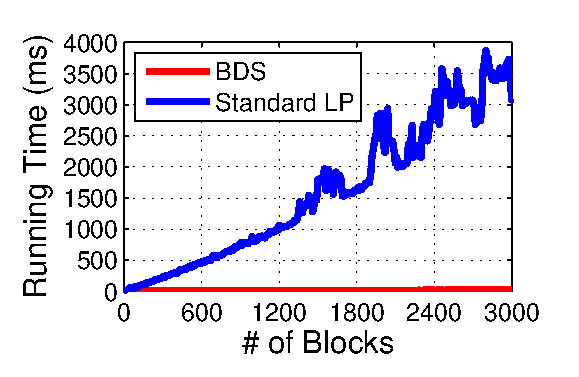
\includegraphics[width=50mm]{images/BDSvsLP.eps} % BDSvsLP.m
%                \caption{Algorithm running time of \name and standard LP.}
%                \label{fig:further:BDSvsLP}
%        \end{subfigure}
%        \begin{subfigure}[b]{0.3\textwidth}
%                \centering
%                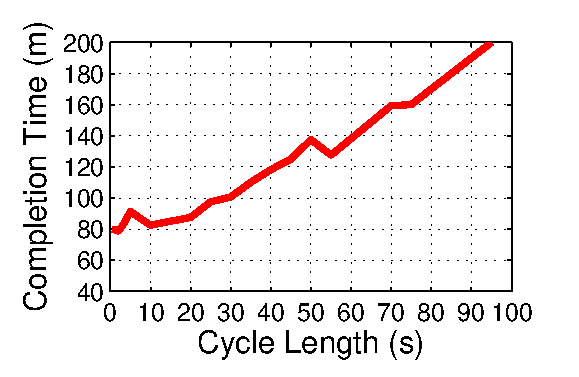
\includegraphics[width=50mm]{images/cycleDiff.eps}%cycleDiff.m
%                \caption{Completion time under different cycle lengths.}
%                \label{fig:further:cycleDiff}
%        \end{subfigure}
%        \begin{subfigure}[b]{0.3\textwidth}
%                \centering
%                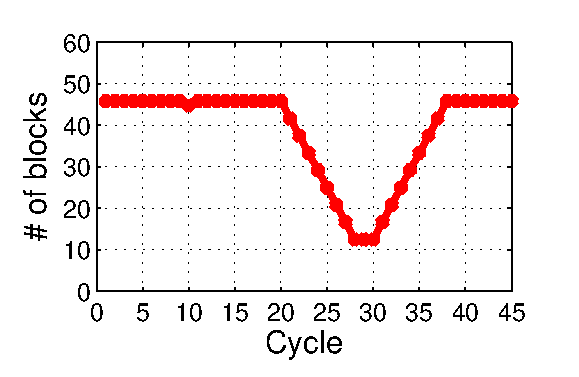
\includegraphics[width=50mm]{images/failure.eps}%fail.m
%                \caption{Average number of downloaded blocks per cycle under failures.}
%                \label{fig:further:failure}
%        \end{subfigure}
%        \caption{Further analysis on (1) running time, (2) cycle length, and (3) fault tolerance.}
%        \label{fig:further}
%\vspace{-0.4cm}
%\end{figure*}



In summary, both the prototype pilot deployment and the trace-driven simulations of \name show 3-5$\times$ speedup over existing solutions, with good scalability and reliability, and near-optimal scheduling results.


%\begin{itemize}
%\item Scalability of centralized control:
%\begin{itemize}
%\item Y: Bandwidth consumption, vs. X: \# of objects
%\item Y: Controller CPU usage, vs. X: \# of objects
%\item Y: Update delay vs. X: \# of objects
%\item Bar-chart to decompose update delay into collecting updates, running algorithm, and updating local agents
%\end{itemize}
%
%\item In-depth analysis:
%\begin{itemize}
%\item A graph to show the tradeoff caused by different update cycles (why 3 seconds is a good tradeoff?)
%\item Reduction on algorithm running time due to the approximation algorithm.
%\item Maybe another graph from the current 6.3?
%\end{itemize}
%
%\item Fault tolerance:
%\begin{itemize}
%\item Y: flow completion time, vs. X: time. Create a toy topology to send objects. The experiment begins with no failure. At time t1, one server is not available, and the graph should show Y only has performance degradation for less than 3 seconds; At time t2, the controller is not available, and the local agent should automatically revert to decentralized local control.
%\end{itemize}
%
%\end{itemize}




